\documentclass[12pt,a4paper]{article}

% PACKAGES
\usepackage[ascii]{inputenc}
\usepackage{amsmath}
\usepackage{amsfonts}
\usepackage{amssymb}
\usepackage{graphicx}

% METADATA
\author{Justin Lee}
\title{Introduction to time series}
\graphicspath{{../images/}}

\begin{document}

\section*{Introduction to time series}
A \textbf{time series} is a collection of observations or values that are indexed by fixed time points. Time time series can be discrcete (known as a discrete-time time series) or continuous (known as a continuous-time time series). Common signals represented by time series include:

\begin{itemize}
	\item speech signals
	\item stock market quotes
	\item Physiological parameters
	\item Dow Jones Industrial Average
	\item EEG and LFP signals
\end{itemize}

Investigations into time series can be broken down into two concepts:\textit{analysis} and \textit{forecasting}. \textit{Time series analysis} involves elucidating the properties that define a particular signal. \textit{Time series forecasting} involves predicting future values and properties of the series in question. Both need to address the underlying statistical properties inherent in the signal. Time series can be analyzed by both \textit{time domain} and \textit{frequency domain} approaches. The \textit{time domain} approach determines the dependence of a current value on past values through parametric modeling. In particular, it draws on regression analysis to fit and make inferences on such models. The \textit{frequency domain} approach uses spectral analysis to explain seasonal (periodic) variations in the data. While it is more appropriate to use time domain methods for short samples, both domains provide tools to analyze any data set.

\subsection*{Examples of time series data}
\paragraph{Australian red wine sales}

\begin{figure}[h]
	\centering
	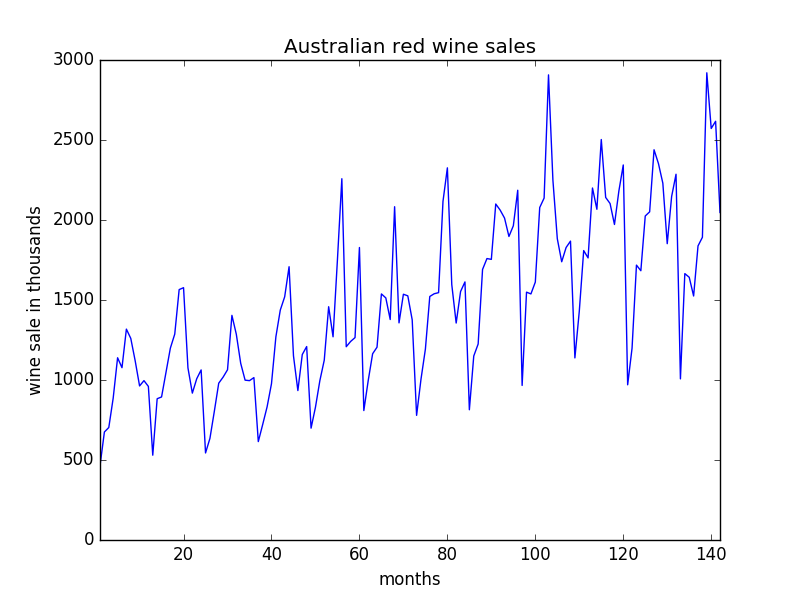
\includegraphics[scale = 0.5]{01_redwine.png}
	\caption{Red wine sales by month from Jan. 1980 to Oct. 1991}
	\label{fig:01_redwine}
\end{figure}

This line plot shows the monthly sales of red wine in Australia from January 1980 to October 1991. There are 142 time points. The graph shows both clear seasonality and an upward trend throughout the time period that the data was sampled from. Image was created in Python. [1].

\paragraph{New York Stock Exchange}

\begin{figure}[h]
	\centering
	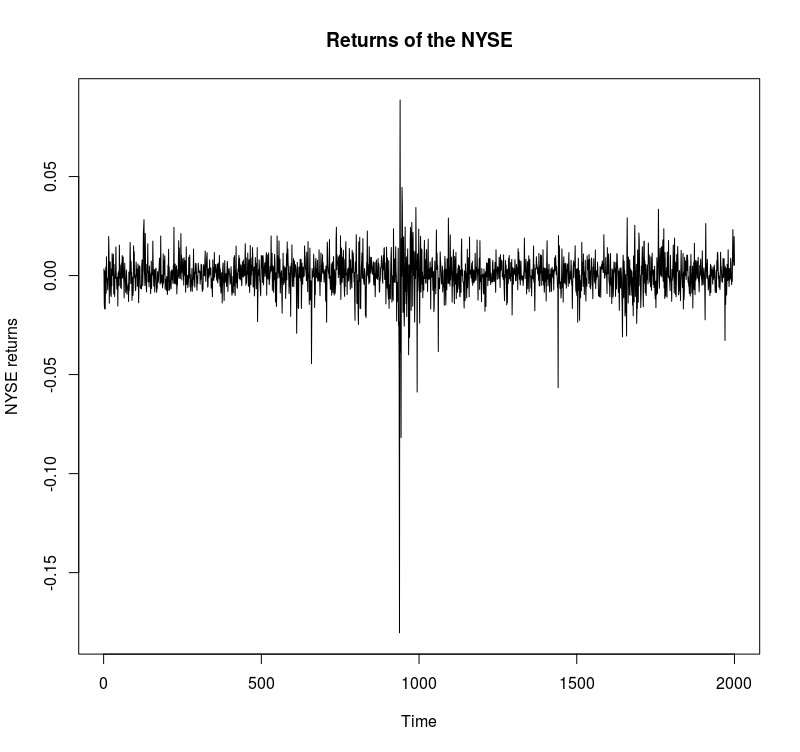
\includegraphics[scale = 0.5]{01_NYSE.png}
	\caption{NYSE returns from February 2, 1984 to December 31, 1991}
	\label{fig:01_NYSE}
\end{figure}

Here are 2000 trading day time points from the New York Stock Exchange. The data runs from February 2, 1984 to December 31, 1991. The values are the daily weighted market returns. There appears to be constant mean. The disturbance towards the middle of the figure represents the crahs of October 19, 1987. Image was created in R. [2].

\subsection*{Time series analysis goals}
The main question to be answered is how to represent the underlying process that generates the data. Once a satisfactory probability model is established, inferences and estimations can be made. Models themselves are made up of 3 components:
\begin{itemize}
	\item trend terms
	\item seasonal terms
	\item a noise term
\end{itemize}
Once these components are identified, they can be individually removed from the data in order to clean up confounding properties. For example, de-noising signals reveal deterministic properties and seasonal adjustments can shed light on long-term patterns. A model is an important tool that gives analysts the most simplistic version of the system while still retaining its key features.

\end{document}